%% ---------------------------------------------------------------------------
%% Copyright (C) 2021 Thomas Lambert <trigon@thl.ovh>
%% Other contributors to this theme are listed here:
%%     https://gitlab.com/thlamb/beamertheme-trigon/-/graphs/master
%%
%% The original template was heavily inspired by Metropolis from Matthias
%% Vogelgesang.
%%
%% License CC-BY-SA 4.0
%% This work is licensed under a Creative Commons Attribution-ShareAlike 4.0
%% International License (https://creativecommons.org/licenses/by-sa/4.0/)
%% ---------------------------------------------------------------------------

\documentclass{ltxdoc}
%\OnlyDescription

\usepackage{xcolor}
\definecolor{tPrim}{HTML}{00707F}   % Green-Blue
\definecolor{tSec}{HTML}{5FA4B0}    % Green-Blue light
\definecolor{tAccent}{HTML}{F07F3C} % Orange
\definecolor{tGrey}{HTML}{E6E6E1}   % Grey-Beige

\usepackage[default,t1,semibold]{sourcesanspro}

\usepackage{parskip}
\usepackage{setspace}
\usepackage{xspace}
\onehalfspacing

%\usepackage{enumitem}
%\setlist[itemize]{noitemsep}
%\setlist[enumerate]{noitemsep}

\usepackage{listings}
\lstset{%
  language=[LaTeX]{TeX},
  basicstyle=\ttfamily,
  keywordstyle=\color{tPrim}\bfseries,
  commentstyle=\color{tSec},
  stringstyle=\color{tSec},
  backgroundcolor=\color{white},
  numbers=none,
  numberstyle=\tiny\ttfamily,
  stepnumber=2,
  showspaces=false,
  showstringspaces=false,
  showtabs=false,
  frame=none,
  framerule=1pt,
  tabsize=2,
  rulesep=5em,
  captionpos=b,
  breaklines=true,
  breakatwhitespace=false,
  framexleftmargin=0em,
  framexrightmargin=0em,
  xleftmargin=0em,
  xrightmargin=0em,
  aboveskip=1em,
  belowskip=1em,
  morekeywords={usetheme,institute,maketitle,@trigon@titleformat,%
  plain,trigonset,setbeamercolor},
}
\lstMakeShortInline|
\usepackage{metalogo}

\setcounter{tocdepth}{2}

\usepackage[colorlinks=true,
linkcolor=tPrim,
menucolor=tPrim,
urlcolor=tPrim]{hyperref}

\setlength{\fboxsep}{0pt}%
\usepackage{caption} % For subfigures
\usepackage{subcaption} % For subfigures

\newcommand{\DescribeOption}[4]{
  \DescribeMacro{#1}
  \begin{minipage}[t]{\textwidth}
    \textit{\textbf{\textcolor{tSec}{#2}}}\dotfill\,#3\par
    \begingroup
    \vspace{0.5em}#4\par
    \endgroup
  \end{minipage}
}


%% ------------------------------------------------------------------------------
\newcommand{\themename}{\textbf{\textsc{Trigon}}\xspace}
\usepackage{readprov}
\ReadPackageInfos{beamerthemetrigon}


%% =============================================================================

\title{\textsc{Trigon}\\ A Modern, elegant and versatile theme for Beamer}
\author{Thomas Lambert \\ \url{trigon@thl.ovh}}
\date{\fileversion~---~\filedate}

%% =============================================================================

\begin{document}

\maketitle
\tableofcontents


%% ------------------------------------
\section{Introduction}

\themename found its origin and inspiration in the graphical guidelines
resulting from the visual identity overhaul of the
\href{https://www.uliege.be}{University of Liège} (Belgium).\\
Although directly inspired from these guidelines, \themename was stripped out of
any mention or specificities related the University and its faculties. This
makes the \themename theme perfectly suitable for many different contexts.

The final product provides a modern, elegant and versatile theme with a
high degree of customization.

\themename's codebase lives on
\href{https://gitlab.com/thlamb/beamertheme-trigon} {Gitlab}. The implementation
of this theme is strongly inspired from the excellent
\href{https://github.com/matze/mtheme}{\textsc{Metropolis}} theme by Matthias
Vogelgesang, from which it borrows numerous options.\newline
Any feature request, issue report or merge requests are welcome.


%% ------------------------------------
\section{Getting Started}

\subsection{Installing from CTAN}
The latest stable version of \themename is available on
\href{https://ctan.org/pkg/beamertheme-trigon}{CTAN} and should now be part of
the usual \TeX\ distibutions (\TeX\ Live, Mac\TeX\ , Mik\TeX\ ), under the name
\textit{beamertheme-trigon}. It means that if your distribution is kept
up-to-date, the package should normally be already installed on your system. If
this is not the case, consider updating the packages of your Tex distribution.

For \TeX\ Live and Mac\TeX\ users, this usually means running
\begin{lstlisting}
tlmgr update --all
\end{lstlisting}
, or if administrative privileges are required
\begin{lstlisting}
sudo tlmgr update --all
\end{lstlisting}

For Mik\TeX\ users, please refer to \href{https://miktex.org/howto/update-miktex}{the official Mik\TeX\ documentation}.


\subsection{Installing from Gitlab}

If you want to use the cutting-edge development version of \themename, you can
install it manually by following these steps:
\begin{description}
  \item[Download the source] from
    \href{https://gitlab.com/thlamb/beamertheme-trigon}{\themename repository}
    using |git clone| or as a \href{https://gitlab.com/thlamb/beamertheme-trigon/-/archive/master/beamertheme-trigon-master.zip}{zip archive} of the latest development version.
  \item[Compile the style files] by running |make sty| inside the downloaded
    directory. (Or run \LaTeX{} directly on |source/trigontheme.ins|.)
  \item[Move the resulting |*.sty| files] to the folder containing your
    presentation. To use \themename with many presentations, run
    |make install| or move the |*.sty| files to a folder in your \TeX{} path
    instead.
  \item[Use the theme] by declaring |\usetheme{trigon}| in the preamble of your
    document.
\end{description}

\themename uses the Make build system to offer the following installation
options for advanced users:

\begin{description}
  \item[|make sty|] builds the theme style files.
  \item[|make doc|] builds this documentation manual.
  \item[|make demo|] builds a demo presentation to test the features of
    \themename.
  \item[|make all|] builds the theme and manual.
  \item[|make clean|] removes the files generated by |make all|.
  \item[|make install|] installs the theme into your local texmf folder.
  \item[|make uninstall|] removes the theme from your local texmf folder.
\end{description}


\subsection{Overleaf}
Since October 2021,
\href{https://www.overleaf.com/blog/tex-live-2021-now-available}{TexLive 2011 is
availabe on Overleaf}. \themename is therefore automatically supported for new
documents. If you want to switch older documents to use the \themename theme,
you need to
\href{https://www.overleaf.com/blog/new-feature-select-your-tex-live-compiler-version}{select
TexLive 2021 or higher as your TeX Live version} (this may cause issues with
other packages used in your presentation).

In addition to that, a template project was created and is publicly availabe in
the
\href{https://www.overleaf.com/latex/templates/trigon-beamer-theme/wjyyzvdzqkgf}{Overleaf
Gallery} to bootstrap your presentation.


\subsection{A Minimal Example}

The following code shows a minimal example of a Beamer presentation using
\themename.

\begin{lstlisting}
\documentclass{beamer}
\usetheme{trigon}       % Use trigon theme
\title{A minimal example}
\subtitle{A subtitle example}
\date{\today}
\author{Thomas Lambert}
\institute{Your university or company}
\begin{document}
  \maketitle
  \section{First Section}
  \begin{frame}{First Frame}
    Hello, world!
  \end{frame}
\end{document}
\end{lstlisting}


\subsection{Dependencies}

\themename depends on the |beamer| class and the following standard packages:
\begin{itemize}
  \item |tikz|
  \item |pgfopts|
\end{itemize}

The theme works best with the open source
\href{https://fonts.adobe.com/fonts/source-sans}{Source Sans Pro} font from
Adobe.\newline
Therefore, the package |sourcesanspro| is loaded by default with the theme.
However, if the user prefers to select an other font, the theme option
|nosourcefonts| can be used to prevent the font package from being loaded.


%% ------------------------------------
\section{Customization}

\subsection{Package options}

\themename provides a number of options, which can be set using a key=value
interface. The primary way to set options is to provide a comma-separated list
of option-value pairs when loading \themename in the preamble:
\begin{lstlisting}
\usetheme[option1=value1, option2=value2, ...]{trigon}
\end{lstlisting}


Options can be changed at any time --- even mid-presentation! --- with the
|\trigonset| macro.
\begin{lstlisting}
\trigonset{option1=newvalue1, option2=newvalue2, ...}
\end{lstlisting}

The list of options is structured as shown in the following example.

\DescribeOption{option key}{list of possible values}{default}{
  A short description of the option.
}

As \themename implementation is heavily inspired from the excellent
\href{https://github.com/matze/mtheme}{\textsc{Metropolis}} theme by Matthias
Vogelgesang, many of \textsc{Metropolis} options are also available in
\themename.

\subsubsection{Main theme}

\DescribeOption{background}{light,dark}{light}{%
  Provides the option to have a dark background and light foreground instead of
  the reverse.
}

\DescribeOption{titleformat}%
{regular, smallcaps, allsmallcaps, allcaps}
{regular}{
  Changes the format of titles, subtitles, section titles, frame titles, and
  the text on ``standout'' frames. The available options produce
  Regular, \textsc{SmallCaps}, \textsc{\MakeLowercase{AllSmallCaps}}, or
  \MakeUppercase{AllCaps} titles. Please refer to
  Section~\ref{sec:titleformats} for known issues with these options.
}

\DescribeOption{usesourcefonts}{true,false}{true}{%
  Chooses if the |sourcesanspro| font package should be loaded |true| or not
  |false|.
}


\subsubsection{Inner theme}

\DescribeOption{sectionpage}{none, simple}{simple}{
  Adds a slide at the start of each section (|simple|). The |none| option
  disables the section page.
}

\DescribeOption{titlestyle}{plain, style1, style2}{style2}{
  Changes the layout of the title page.
}
\begin{figure}[h!]
  \begin{subfigure}[b]{0.3\textwidth}
    \fbox{
\includegraphics[width=\textwidth]{screenshots/layout_example-02.jpg}}
    \caption*{plain}
  \end{subfigure}
  \hspace{\fill}
  \begin{subfigure}[b]{0.3\textwidth}
    \fbox{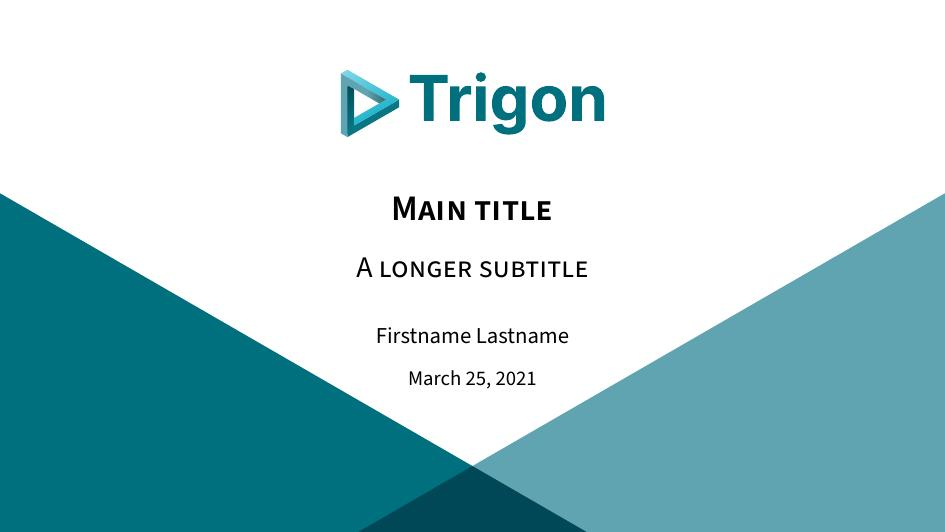
\includegraphics[width=\textwidth]{screenshots/layout_example-03.jpg}}
    \caption*{style1}
  \end{subfigure}
  \hspace{\fill}
  \begin{subfigure}[b]{0.3\textwidth}
    \fbox{
\includegraphics[width=\textwidth]{screenshots/layout_example-01.jpg}}
    \caption*{style2 (default)}
  \end{subfigure}
\end{figure}

\DescribeOption{sectionstyle}{plain, style1, style2, style3}{plain}{
  Changes the layout of the section page. |style3| is similar to |plain| but
  with the right triangle in grey instead of theme color.
}
\begin{figure}[h!]
  \begin{subfigure}[b]{0.3\textwidth}
    \fbox{\includegraphics[width=\textwidth]{screenshots/layout_example-04.jpg}}
    \caption*{plain (default)}
  \end{subfigure}
  \hspace{\fill}
  \begin{subfigure}[b]{0.3\textwidth}
    \fbox{\includegraphics[width=\textwidth]{screenshots/layout_example-05.jpg}}
    \caption*{style1}
  \end{subfigure}
  \hspace{\fill}
  \begin{subfigure}[b]{0.3\textwidth}
    \fbox{\includegraphics[width=\textwidth]{screenshots/layout_example-06.jpg}}
    \caption*{style2}
  \end{subfigure}
\end{figure}

\DescribeOption{slidestyle}{blank, style1, cyber}{blank}{
  Changes the background of the regular frames.
}
\begin{figure}[h!]
  \hspace{\fill}
  \begin{subfigure}[b]{0.3\textwidth}
    \fbox{\includegraphics[width=\textwidth]{screenshots/layout_example-08.jpg}}
    \caption*{blank (default)}
  \end{subfigure}
  \hspace{\fill}
  \begin{subfigure}[b]{0.3\textwidth}
    \fbox{\includegraphics[width=\textwidth]{screenshots/layout_example-09.jpg}}
    \caption*{style1}
  \end{subfigure}
  \hspace{\fill}
  \begin{subfigure}[b]{0.3\textwidth}
    \fbox{\includegraphics[width=\textwidth]{screenshots/layout_example-10.jpg}}
    \caption*{cyber}
  \end{subfigure}
\end{figure}

\subsubsection{Outer theme}

\DescribeOption{numbering}{none, counter, fraction}{counter}{
  Controls whether the frame number at the bottom right of each slide is
  omitted (|none|), shown (|counter|) or displayed as a fraction of the total
  number of frames (|fraction|).
}

\subsubsection{Color theme}
\DescribeOption{block}{transparent, fill}{fill}{
  Optionally adds a light grey background to block environments like |theorem|
  and |example|.
}

\DescribeOption{headingcolor}{default, theme}{default}{
  Controls weather the color of all headings (title page, frame title, etc.)
  should be in black (|default|) or in a slightly darker shade of the theme
  color |theme|.
}

\DescribeOption{textgcolor}{default, theme}{default}{
  Controls weather the color of the regular text elements should be in black
  (|default|) or in a slightly darker shade of the theme color |theme|.
}

\subsubsection{Font theme}

\DescribeMacro{titleformat title}
\DescribeMacro{titleformat subtitle}
\DescribeMacro{titleformat section}
\DescribeOption{titleformat frame}%
{regular, smallcaps, allsmallcaps, allcaps}%
{regular}{
  Individually controls the format of titles, subtitles, section titles, and
  frame titles (see |titleformat|, above).
}


\subsection{Color Customization}

The included \themename color theme is used by default, but its colors can be
easily changed to suit your tastes. All of the theme's styles are defined in
terms of a few main colors:
\begin{itemize}
  \item |tPrim| The primary theme color, used for main triangle elements, and
    for headings and text if the appropriate options are selected.
  \item |tSec| The secondary theme color (lighter shade of the primary color),
    used for some triangle elements and example text.
  \item |tAccent| The accent color, used mostly for alerted text.
  \item |tGrey| A grey color, used for background elements (triangles, blocks,
    etc.).
  \item |tTxt| The default text color.
  \item |tBg| The default background color.
  \item |tGreyBg| A tint of grey to use for the triangle elements.
  \item |tTheme| A tint of the |tPrim| color to use for some triangle elements.
\end{itemize}

An easy way to customize the theme is to redefine these colors using

\begin{lstlisting}
  \colorlet{tPrim}{ ... }
  \colorlet{tSec}{ ... }
  ...
\end{lstlisting}
in your preamble.

\subsection{Logos}

The package allows the inclusion of logos on the title page and on the content
slides. For that, the following commands are defined:
\begin{lstlisting}
  \biglogo[<options>]{path/to/your/titlepage_logo}
  \smalllogo[<options>]{path/to/your/titlepage_logo}
\end{lstlisting}
These two commands are just replacements for |\includegraphics| and they will
pass the options as-is so you can perfectly size and position the images.



\section{Tips \& Tricks}

\subsection{Backup Slides}

Speakers will often include extra slides at the end of their presentation to
refer to during audience questions. One easy way to do this is to include the
\verb|appendixnumberbeamer| package in your preamble and call \verb|\appendix|
before your backup slides.

\themename will automatically turn off slide numbering for slides in the
appendix.


\section{Known Issues}

\subsection{Title formats}
\label{sec:titleformats}

Be aware that not every font supports small caps, so the |smallcaps| or
|allsmallcaps| options may not work if you use a font other than
|sourcesanspro|.

The title format options |allsmallcaps| and |allcaps| are quite nice from an
aesthetic point of view, but their use of |\MakeLowercase| and
|\MakeUppercase| can cause unexpected problems. For example:

\begin{itemize}
  \item Some commands, like |\\|, do not work inside |\MakeLowercase| and
    |\MakeUppercase|. (See \textsc{Metropolis}
    \href{https://github.com/matze/mtheme/issues/125} {\#125})
  \item Only alphabetic characters are affected by |\MakeLowercase|, so
    numerals and punctuation remain at full height. This can spoil some of the
    aesthetic benefits of |allsmallcaps|. (See \textsc{Metropolis}
    \href{https://github.com/matze/mtheme/issues/33}{\#33})
  \item |\MakeLowercase| and |\MakeUppercase| apply to math mode and
    |\scshape| does not. This can easily introduce mathematical errors that
    are hard to catch.
  \item It is impossible to typeset symbols which are encoded as uppercase
    letters in a different font. In particular, |\mathbb| and |\mathcal|
    letters will be replaced by other math glyphs. (See \textsc{Metropolis}
    \href{https://github.com/matze/mtheme/issues/153}{\#153})
\end{itemize}

The |allsmallcaps| and |allcaps| options are safe to use if your titles contain
only alphabetic characters and do not require the expansion of any macros.


\section{License}
\themename is licensed under the terms of the
\href{https://creativecommons.org/licenses/by-sa/4.0/}{Creative Commons
Attribution-ShareAlike 4.0} license.


\section{Implementation}
\DocInput{beamerthemetrigon.dtx}
\DocInput{beamerinnerthemetrigon.dtx}
\DocInput{beamerouterthemetrigon.dtx}
\DocInput{beamerfontthemetrigon.dtx}
\DocInput{beamercolorthemetrigon.dtx}

\end{document}

